%%
% Report for Assignment I, based on the TUM article template
% (https://gitlab.lrz.de/latex4ei/tum-templates).
% Build: latexmk (reads ./latexmkrc so the class files in tum/ are found).
% Figures come from ../figures (written by src/*.py), tables from ../results.
%%

\documentclass[
  english,
  font=times,
  twocolumn,
]{tumarticle}

\usepackage{cite}
\usepackage{booktabs}

% generated artefacts live outside report/
\graphicspath{{../figures/}}
\newcommand{\resultsdir}{../results}
\newcommand{\repourl}{\url{https://github.com/maxmchl/BPI-17-Challenge}}

\title{First Assignment - Business Process Prediction, Simulation, and Optimization - Summer Semester 2026}
\subtitle{Process and Data Science on the BPIC-17 Event Log}

\author[email=maximilian.michel@tum.de]{Maximilian Michel}

\date\today

\begin{document}

\maketitle

\begin{abstract}
% TODO: task, log, findings, main results in 4-5 sentences.
\end{abstract}

\section{Introduction}
% TODO: application domain, when/why the log was generated, the process it captures,
% existing BPIC'17 reports and their key insights.

\section{Approach and Results}
% TODO: approach overview.
Code: \repourl

\subsection{Technical Setup and Preliminaries}
% TODO: libraries, visualization, modeling tools; one footnote per tool, e.g.
% PM4Py\footnote{\tiny PM4Py \url{https://pm4py.fit.fraunhofer.de}}

\subsection{Simple Event Log Analysis}
% TODO: text; table generated by src/stats.py

\begin{table}[h]
    \caption{Basic event log statistics.}  % TODO: caption
    \centering
    \small
    \renewcommand{\arraystretch}{1.2}
    \input{\resultsdir/basic_stats.tex}
    \label{tab:statistics}
\end{table}

\begin{figure}[t]
    \centering
    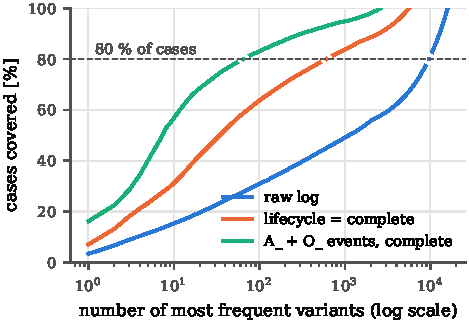
\includegraphics[width=\columnwidth]{variant_coverage.pdf}
    \caption{TODO}
    \label{fig:variant_coverage}
\end{figure}

\begin{figure}[t]
    \centering
    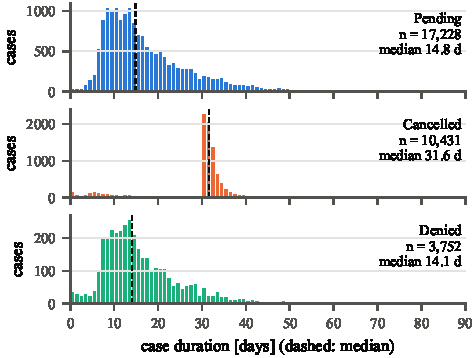
\includegraphics[width=\columnwidth]{duration_by_outcome.pdf}
    \caption{TODO}
    \label{fig:duration_by_outcome}
\end{figure}

\begin{figure}[t]
    \centering
    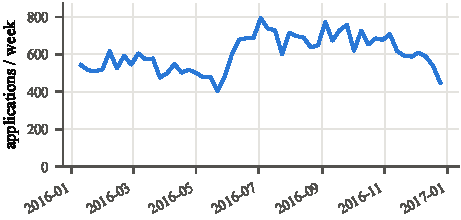
\includegraphics[width=\columnwidth]{weekly_arrivals.pdf}
    \caption{TODO}
    \label{fig:weekly_arrivals}
\end{figure}

\subsection{Process Model Creation and Validation}

\subsubsection{Process Discovery}
% TODO: >= 2 discovery algorithms; models go to the appendix.

\subsubsection{Quality Metrics}
% TODO: all PM4Py metrics (token replay vs alignments, runtimes) + 2 own simplicity metrics.

\subsubsection{Final Process Model}
% TODO: iteration log, design decisions, trade-offs, final BPMN 2.0 + all metrics.
% \begin{figure*}[t]
%     \centering
%     \includegraphics[width=\textwidth]{final_bpmn.pdf}
%     \caption{TODO}
%     \label{fig:bpmn}
% \end{figure*}

\subsubsection{Decision Mining}
% TODO: decision block per XOR (alignment-based), DT vs MLP + SHAP, BPMN with rules.

\subsection{Advanced Analysis}
% TODO: hypothesis, approach and result, interpretation.

\section*{Declaration of GenAI Usage}
% TODO: tools used and for what.

\nocite{*}  % TODO: remove once the text cites the references
\bibliographystyle{plain}
\bibliography{references}

\appendix
\onecolumn
\section{Discovered Process Models}
% TODO: models from the discovery algorithms.

\end{document}
